\begin{figure}[!h]
\centerline{\bfseries\large High-Density Workload : Trials 1--3}\\
\fbox{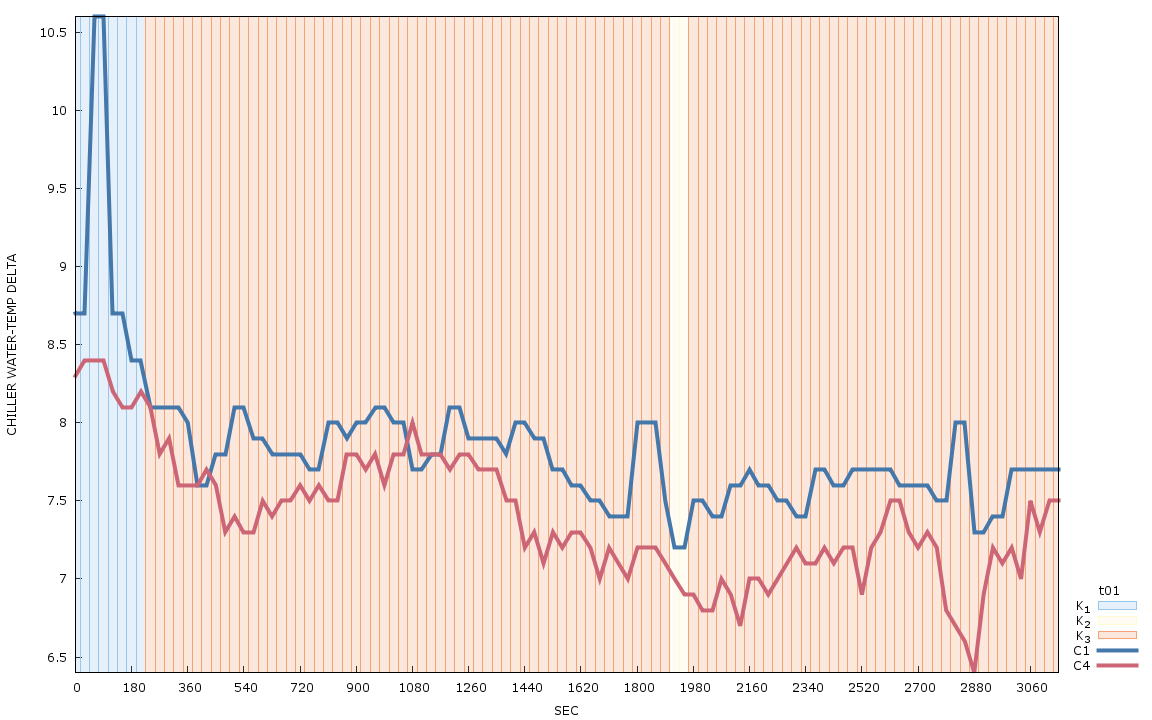
\includegraphics[bb=0 0 1152 720, width=15in]{cluster3/hd/CH_WTD/CH_WTD_t01.png}}
\fbox{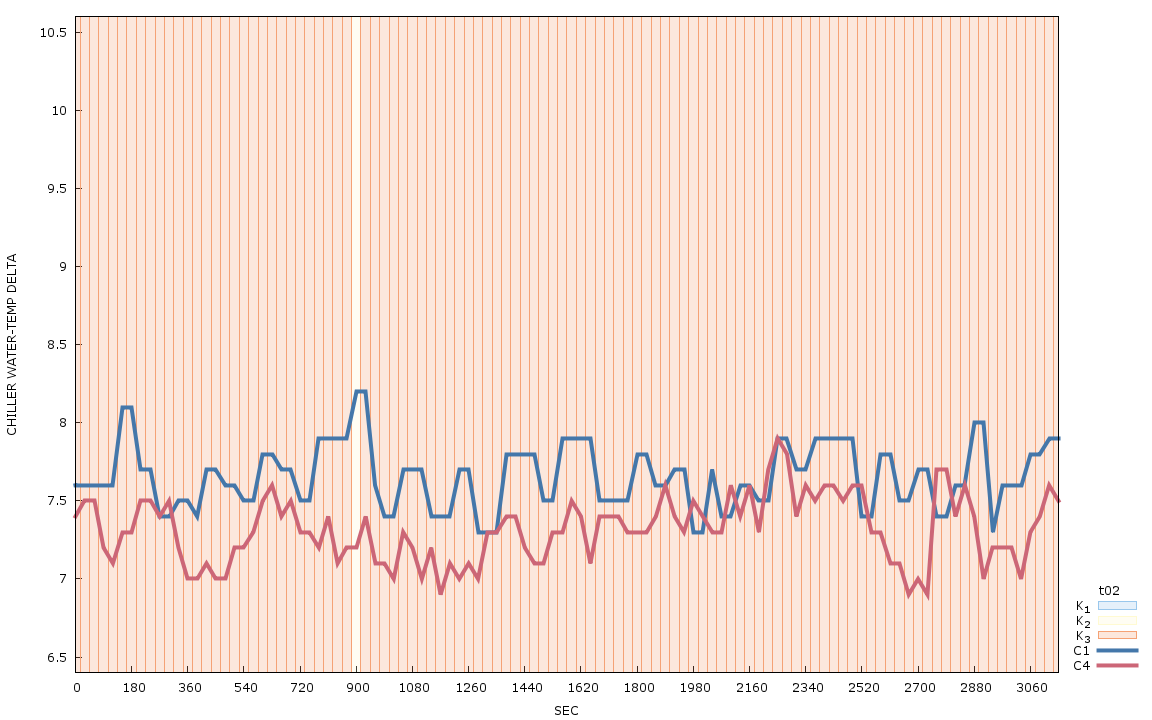
\includegraphics[bb=0 0 1152 720, width=15in]{cluster3/hd/CH_WTD/CH_WTD_t02.png}}
\fbox{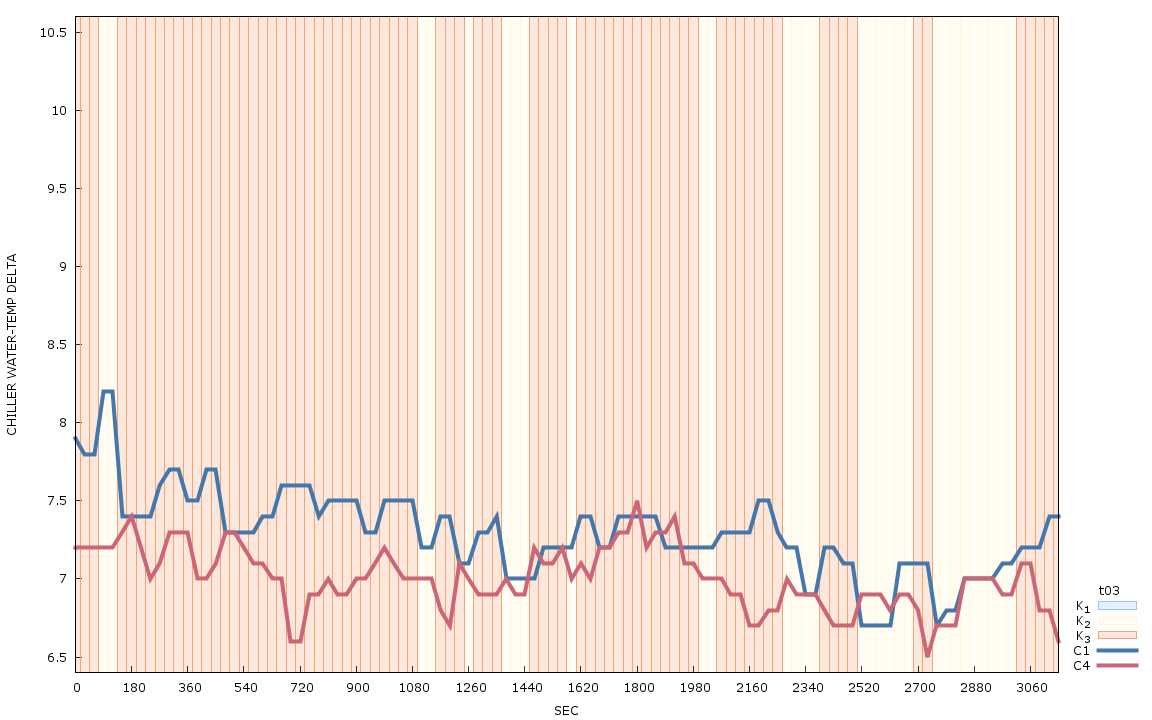
\includegraphics[bb=0 0 1152 720, width=15in]{cluster3/hd/CH_WTD/CH_WTD_t03.png}}
\caption{Chiller units C1 and C4; EM clustering across all three trials with $k=3$.}
\end{figure}
\begin{figure}[!h]
\centerline{\bfseries\large High-Density Workload : Trials 1--3}\\
\fbox{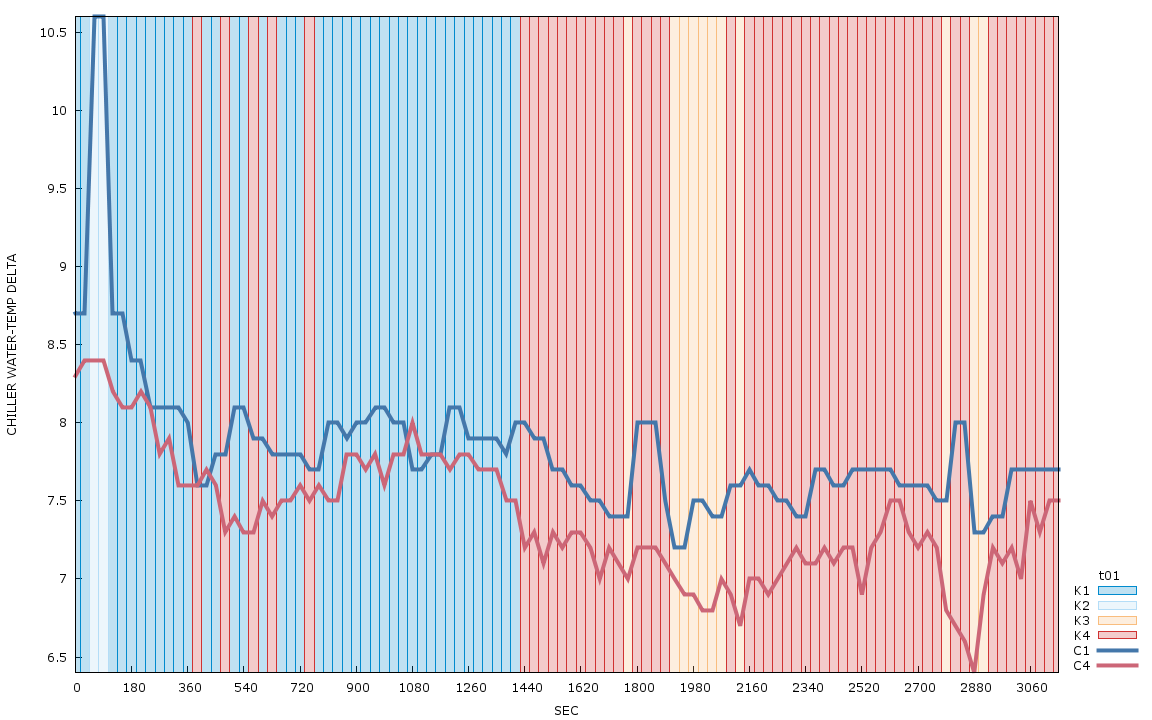
\includegraphics[bb=0 0 1152 720, width=15in]{cluster4/hd/CH_WTD/CH_WTD_t01.png}}
\fbox{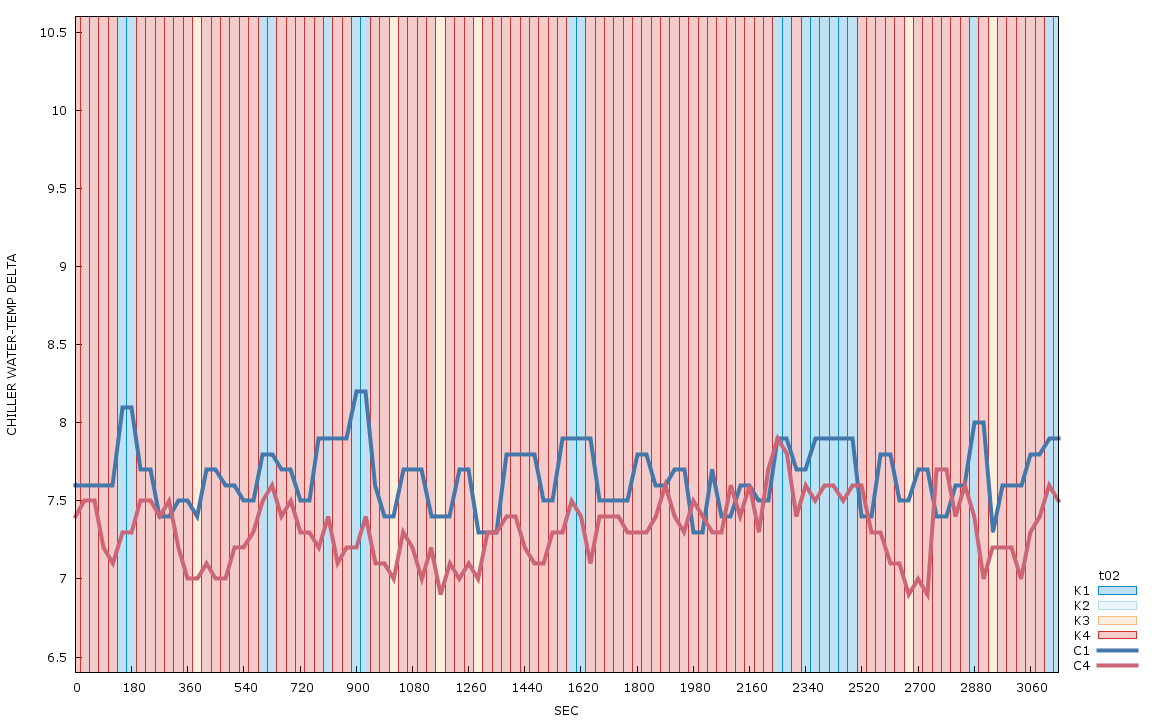
\includegraphics[bb=0 0 1152 720, width=15in]{cluster4/hd/CH_WTD/CH_WTD_t02.png}}
\fbox{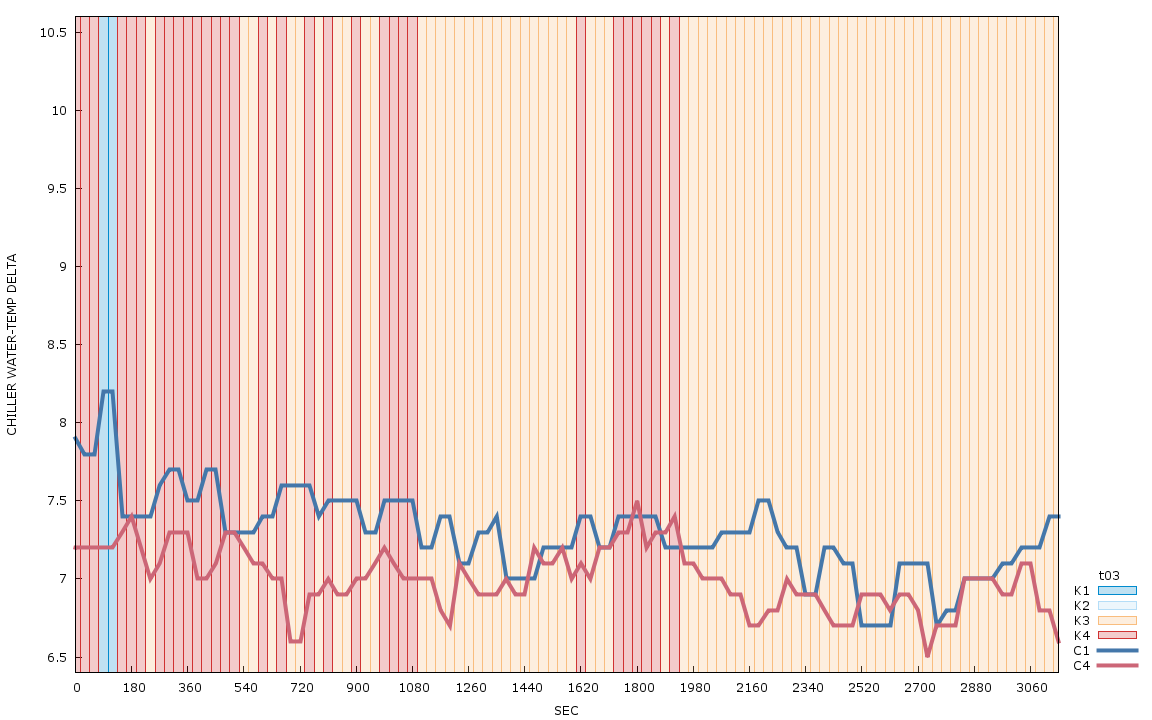
\includegraphics[bb=0 0 1152 720, width=15in]{cluster4/hd/CH_WTD/CH_WTD_t03.png}}
\caption{Chiller units C1 and C4; K-Means clustering across all three trials with $k=4$.}
\end{figure}
\begin{figure}[!h]
\centerline{\bfseries\large High-Density Workload : Trials 1--3}\\
\fbox{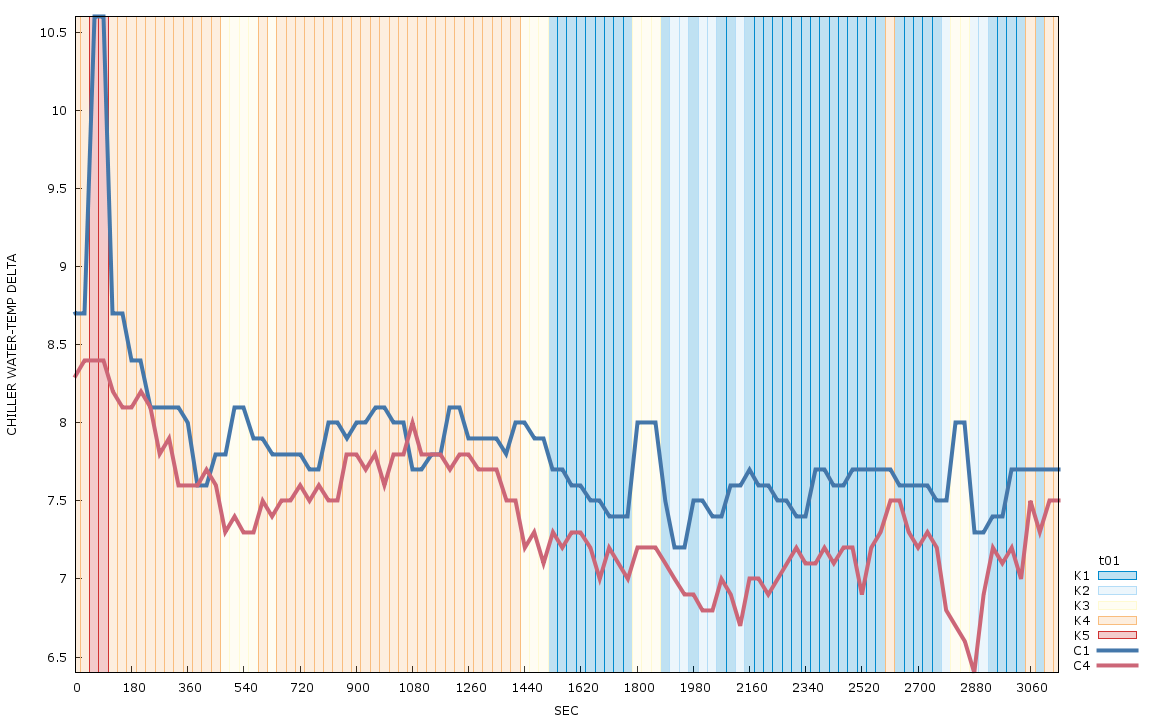
\includegraphics[bb=0 0 1152 720, width=15in]{cluster5/hd/CH_WTD/CH_WTD_t01.png}}
\fbox{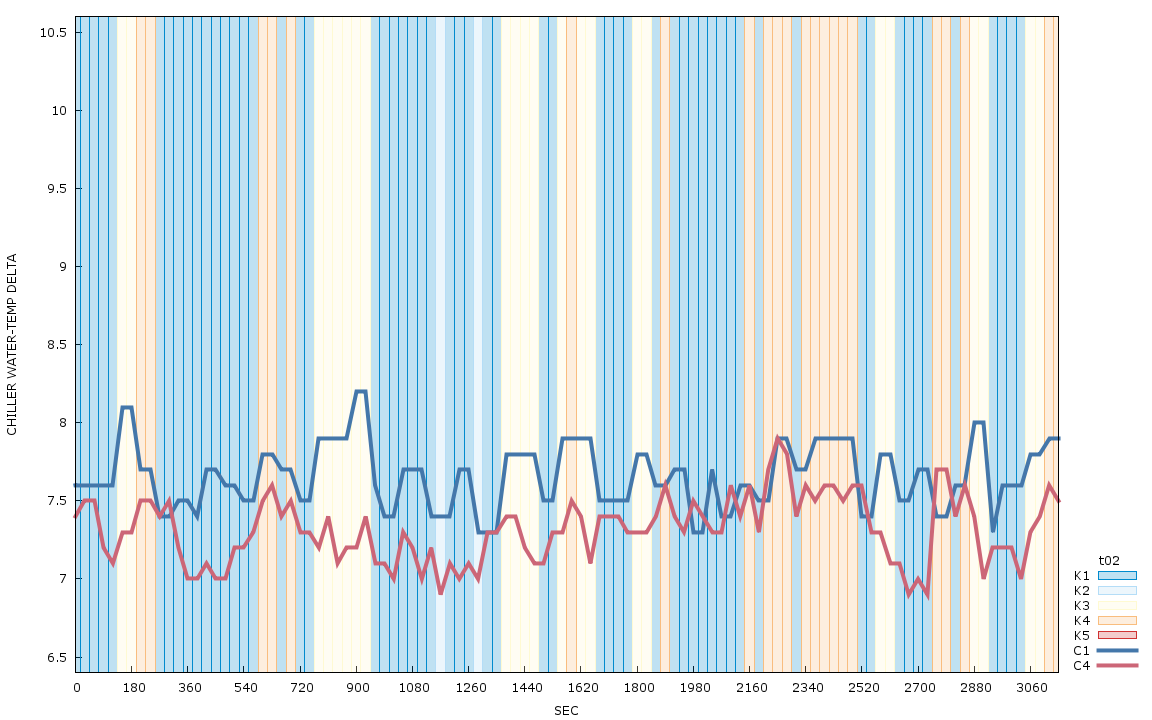
\includegraphics[bb=0 0 1152 720, width=15in]{cluster5/hd/CH_WTD/CH_WTD_t02.png}}
\fbox{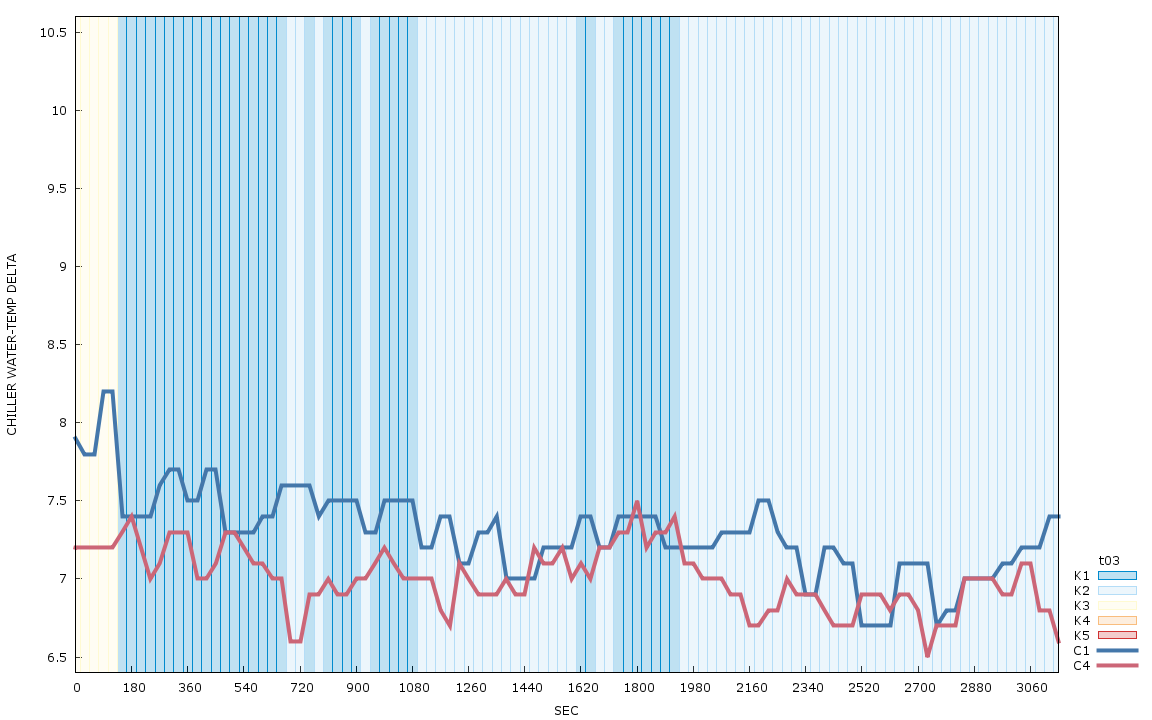
\includegraphics[bb=0 0 1152 720, width=15in]{cluster5/hd/CH_WTD/CH_WTD_t03.png}}
\caption{Chiller units C1 and C4; K-Means clustering across all three trials with $k=5$.}
\end{figure}
\begin{figure}[!h]
\centerline{\bfseries\large High-Density Workload : Trials 1--3}\\
\fbox{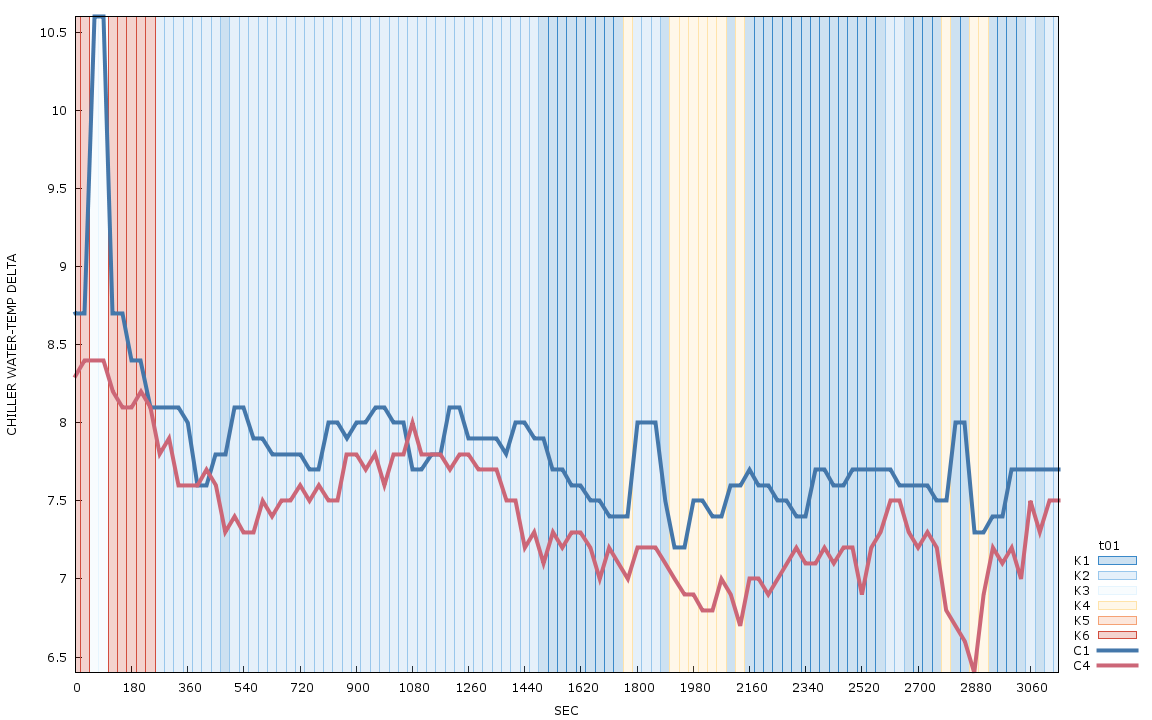
\includegraphics[bb=0 0 1152 720, width=15in]{cluster6/hd/CH_WTD/CH_WTD_t01.png}}
\fbox{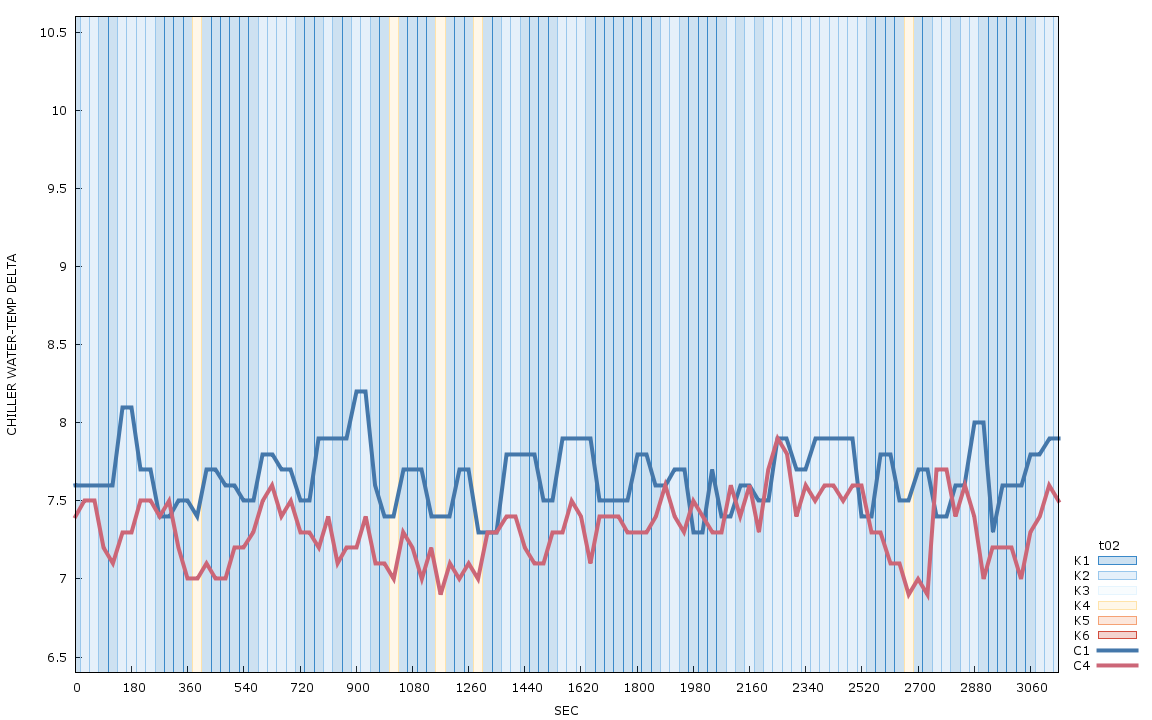
\includegraphics[bb=0 0 1152 720, width=15in]{cluster6/hd/CH_WTD/CH_WTD_t02.png}}
\fbox{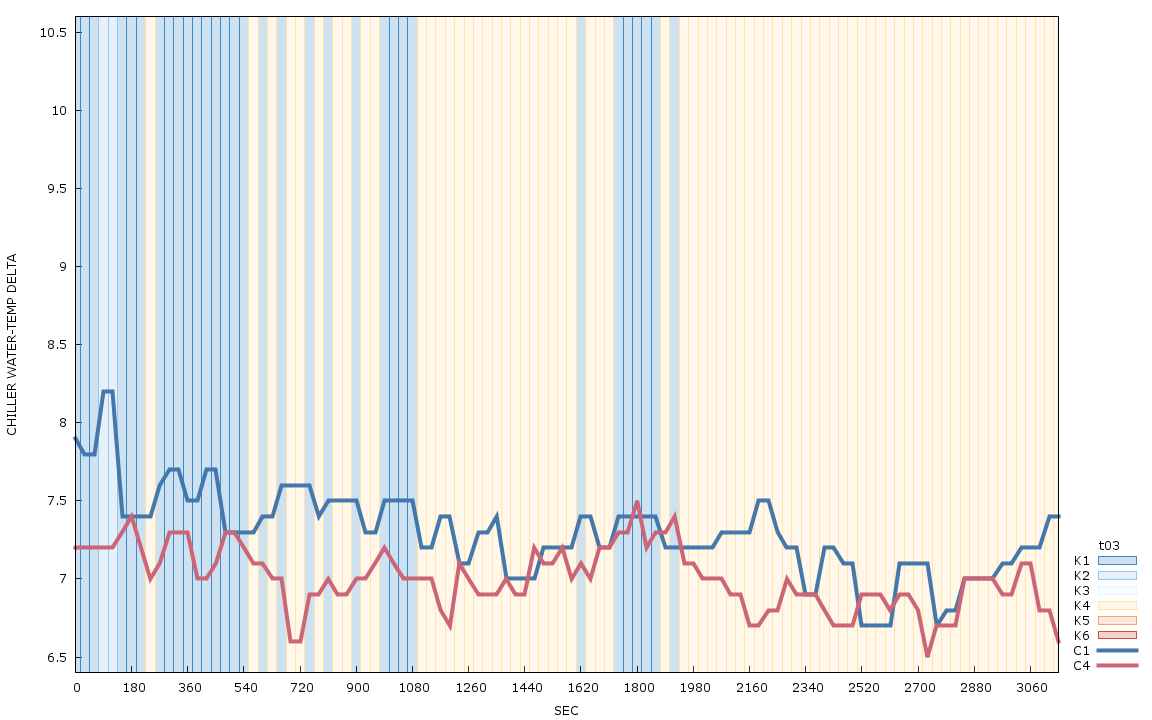
\includegraphics[bb=0 0 1152 720, width=15in]{cluster6/hd/CH_WTD/CH_WTD_t03.png}}
\caption{Chiller units C1 and C4; K-Means clustering across all three trials with $k=6$.}
\end{figure}
\begin{figure}[!h]
\centerline{\bfseries\large High-Density Workload : Trials 1--3}\\
\fbox{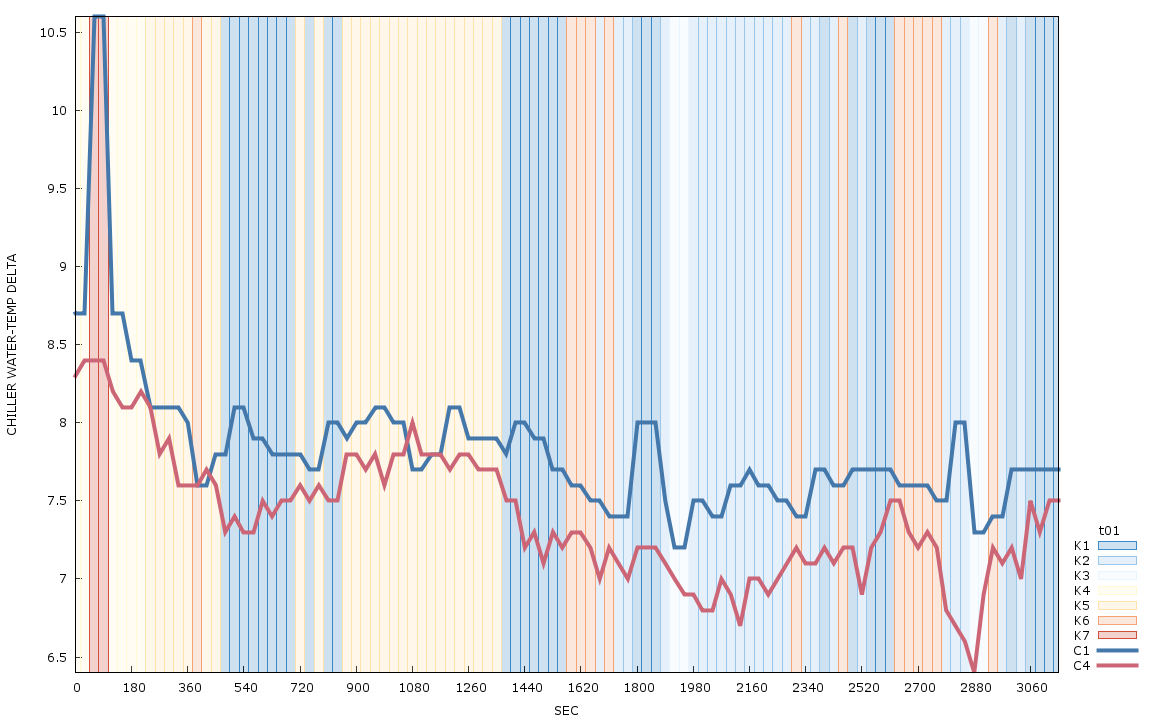
\includegraphics[bb=0 0 1152 720, width=15in]{cluster7/hd/CH_WTD/CH_WTD_t01.png}}
\fbox{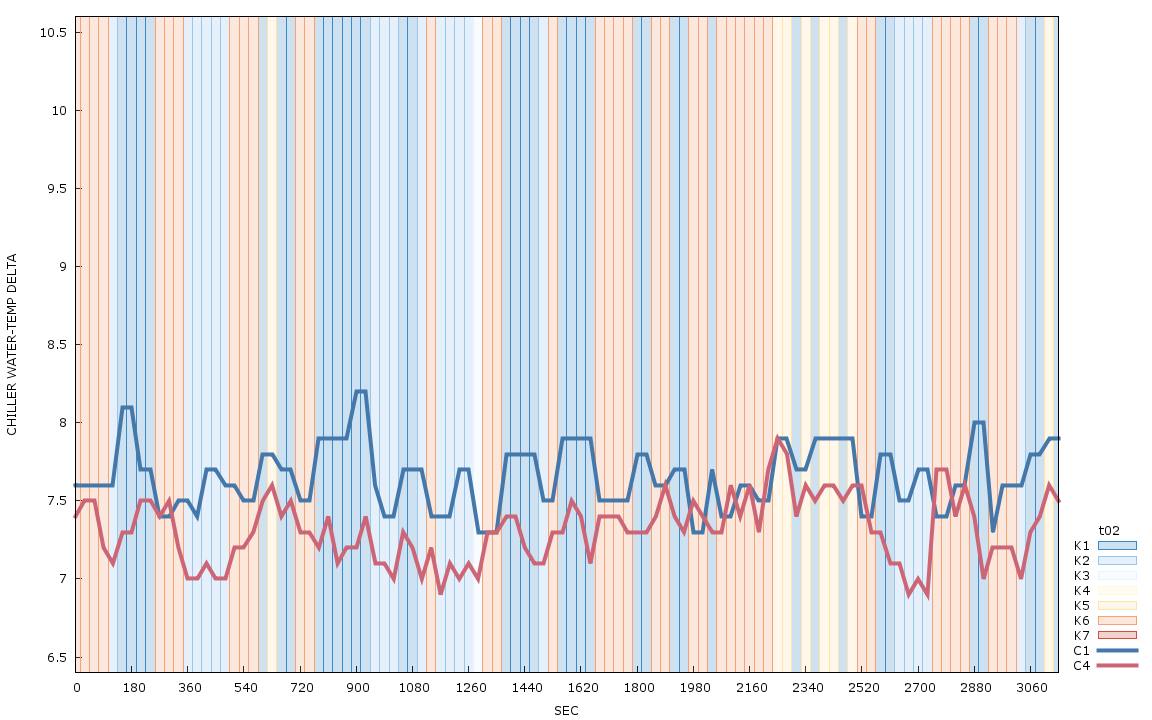
\includegraphics[bb=0 0 1152 720, width=15in]{cluster7/hd/CH_WTD/CH_WTD_t02.png}}
\fbox{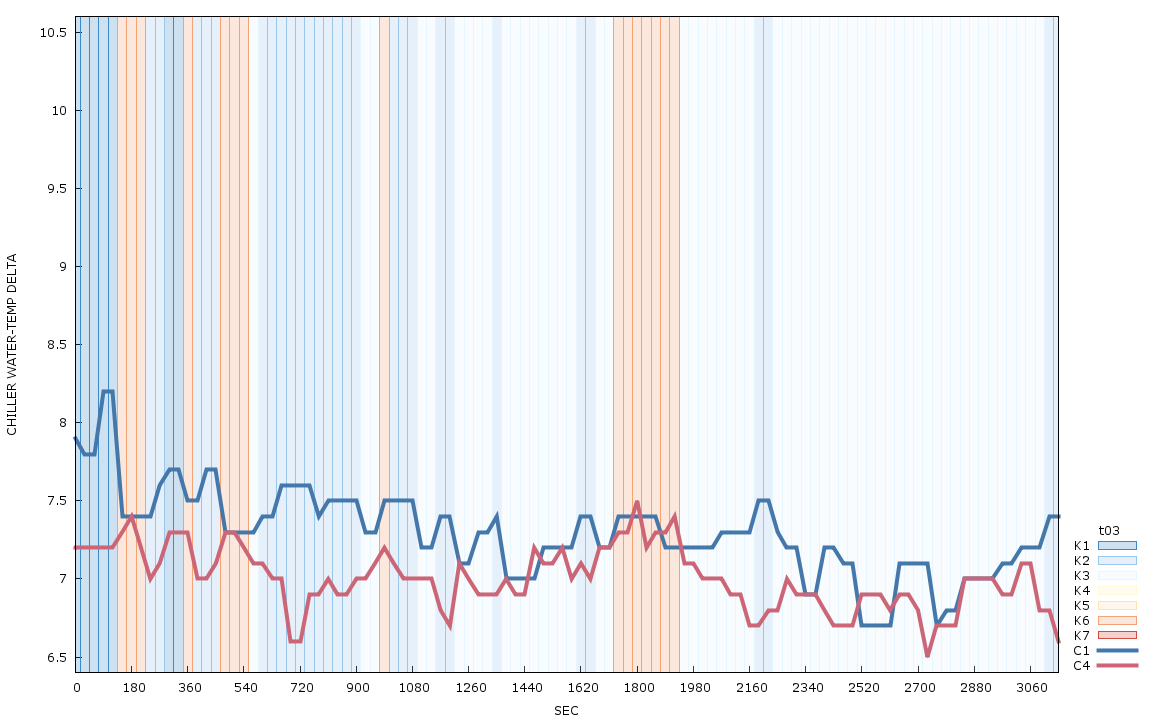
\includegraphics[bb=0 0 1152 720, width=15in]{cluster7/hd/CH_WTD/CH_WTD_t03.png}}
\caption{Chiller units C1 and C4; K-Means clustering across all three trials with $k=7$.}
\end{figure}
\begin{figure}[!h]
\centerline{\bfseries\large High-Density Workload : Trials 1--3}\\
\fbox{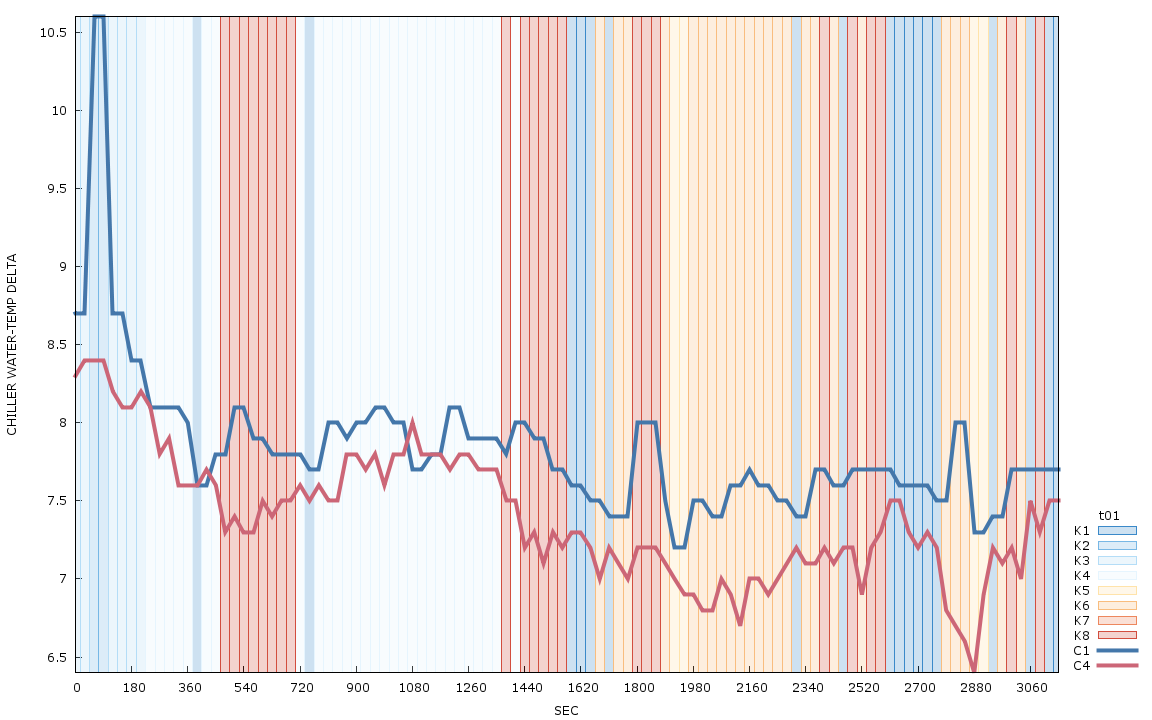
\includegraphics[bb=0 0 1152 720, width=15in]{cluster8/hd/CH_WTD/CH_WTD_t01.png}}
\fbox{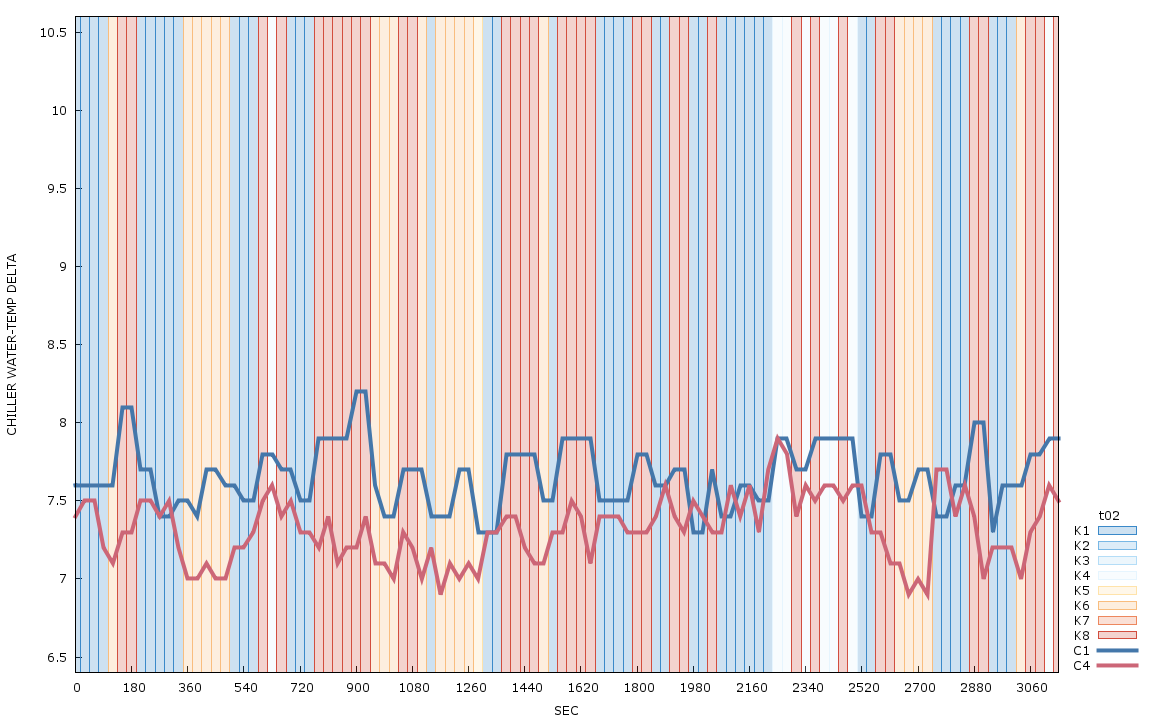
\includegraphics[bb=0 0 1152 720, width=15in]{cluster8/hd/CH_WTD/CH_WTD_t02.png}}
\fbox{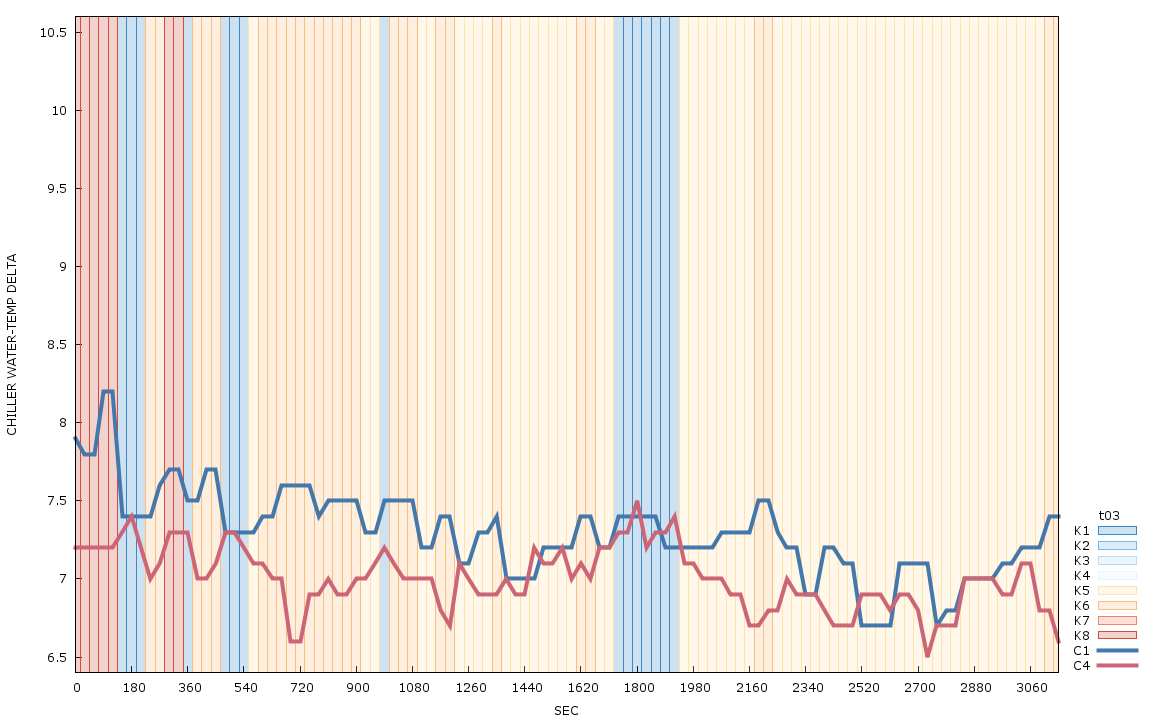
\includegraphics[bb=0 0 1152 720, width=15in]{cluster8/hd/CH_WTD/CH_WTD_t03.png}}
\caption{Chiller units C1 and C4; K-Means clustering across all three trials with $k=8$.}
\end{figure}
\begin{figure}[!h]
\centerline{\bfseries\large High-Density Workload : Trials 1--3}\\
\fbox{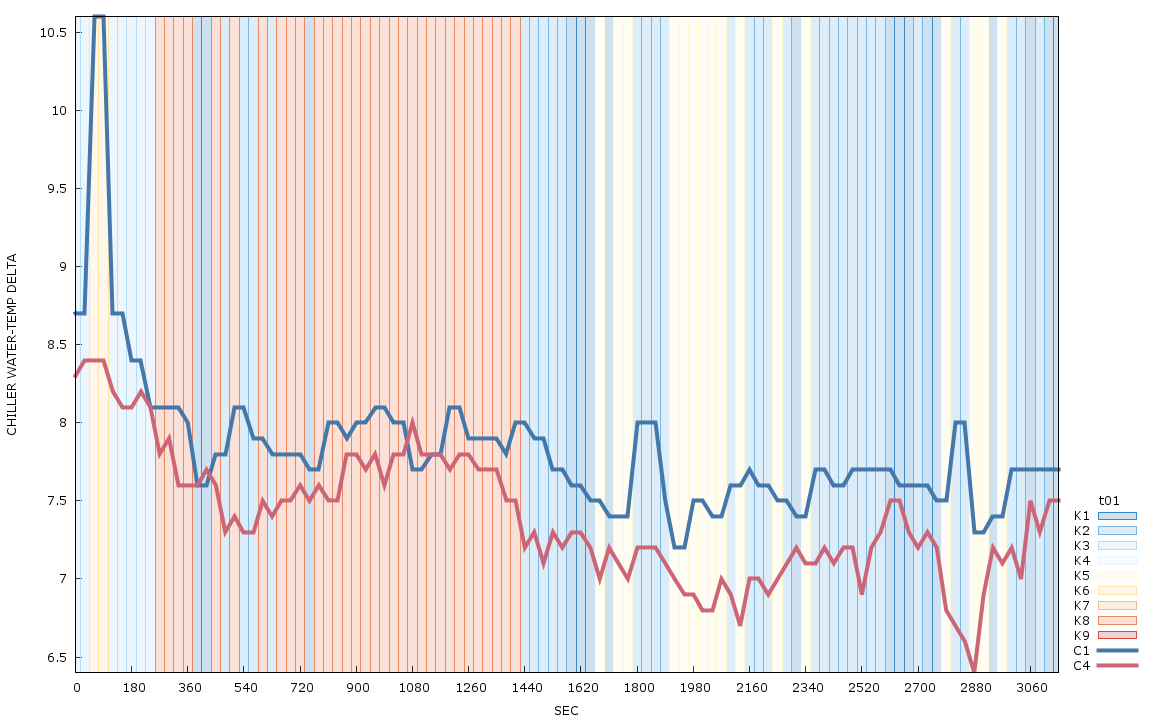
\includegraphics[bb=0 0 1152 720, width=15in]{cluster9/hd/CH_WTD/CH_WTD_t01.png}}
\fbox{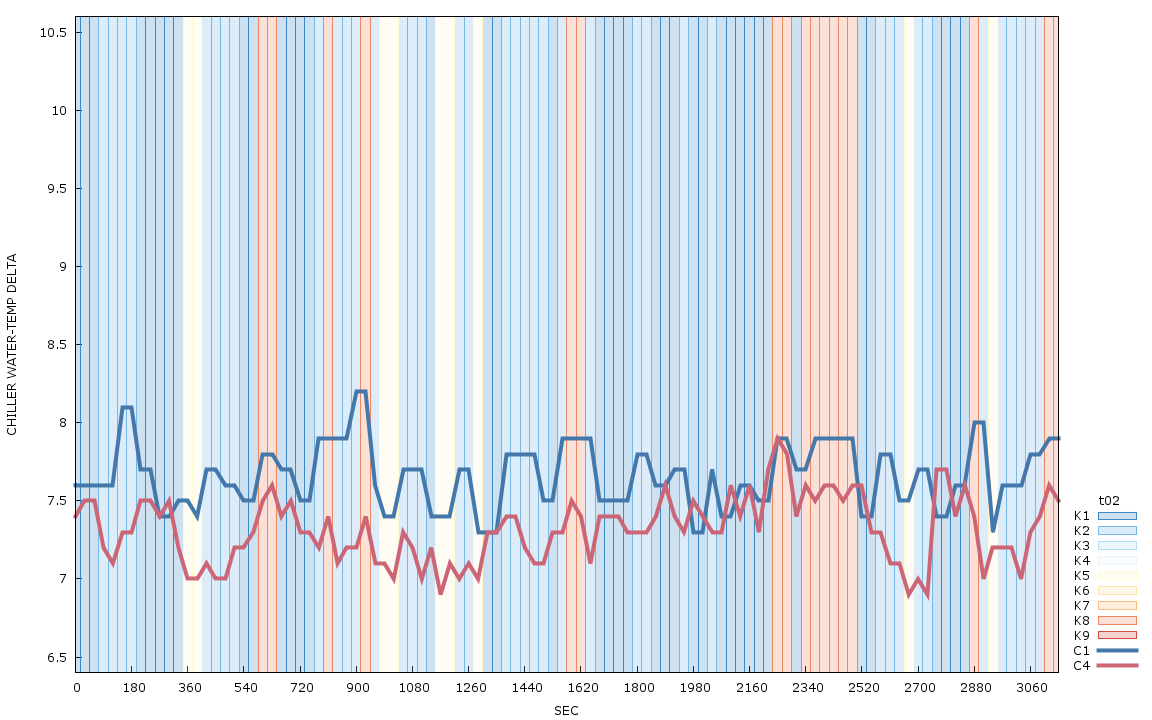
\includegraphics[bb=0 0 1152 720, width=15in]{cluster9/hd/CH_WTD/CH_WTD_t02.png}}
\fbox{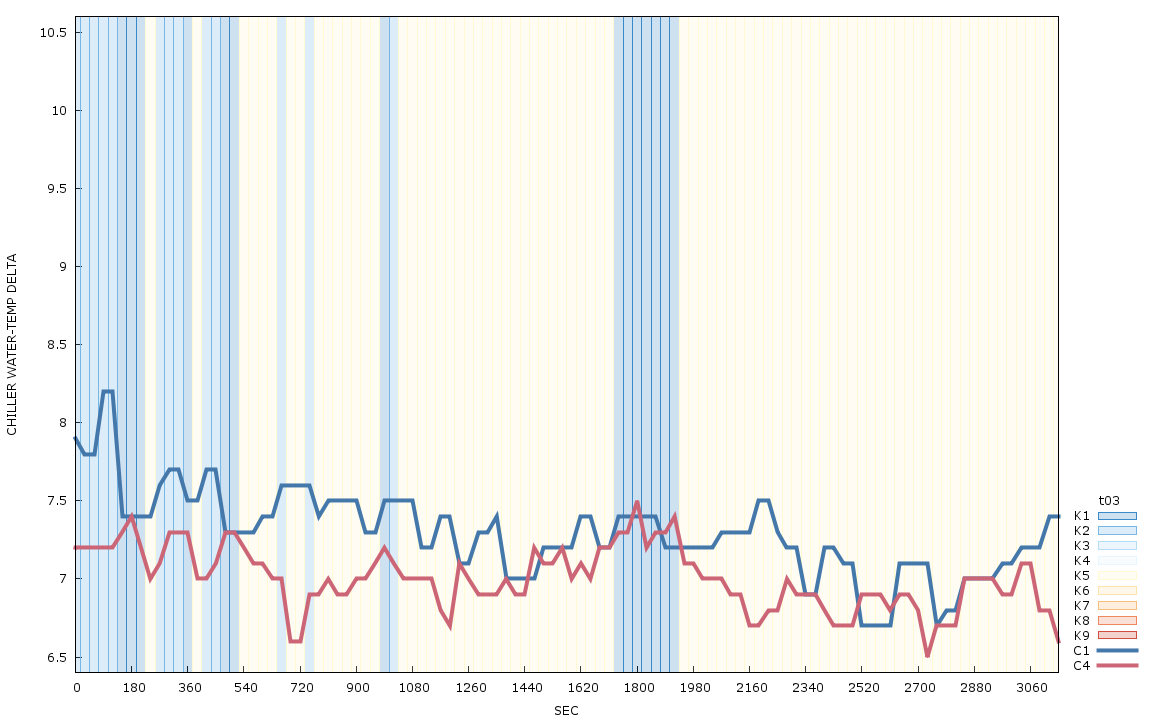
\includegraphics[bb=0 0 1152 720, width=15in]{cluster9/hd/CH_WTD/CH_WTD_t03.png}}
\caption{Chiller units C1 and C4; K-Means clustering across all three trials with $k=9$.}
\end{figure}
\begin{figure}[!h]
\centerline{\bfseries\large High-Density Workload : Trials 1--3}\\
\fbox{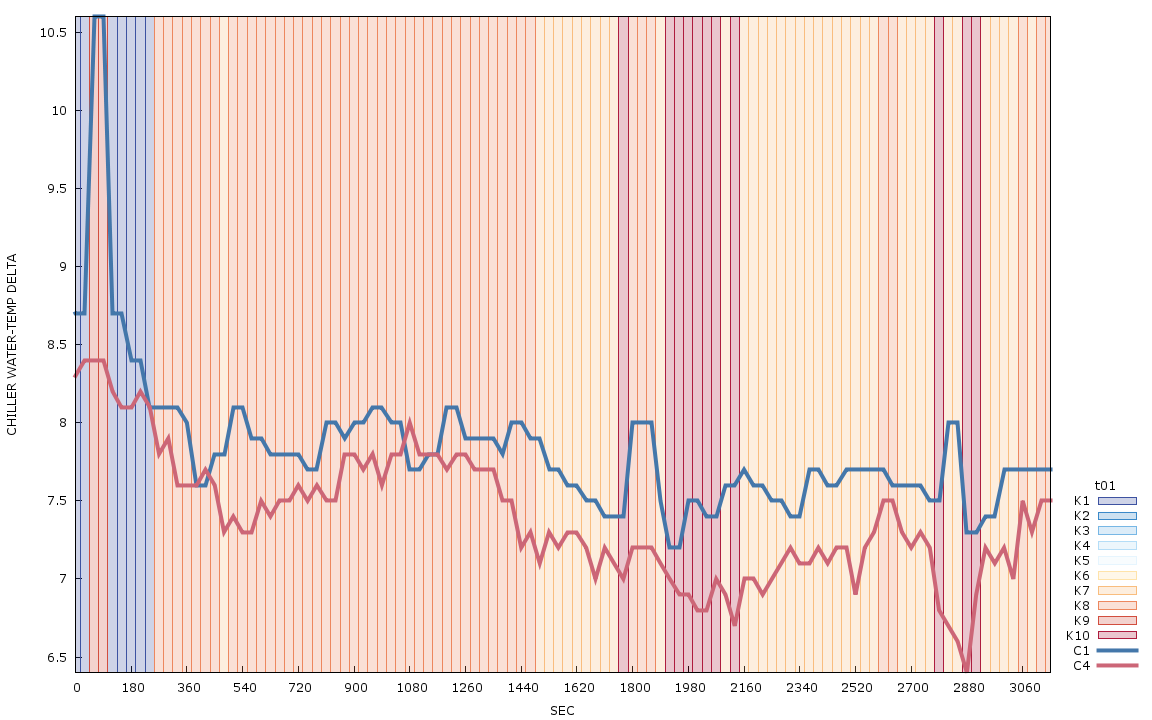
\includegraphics[bb=0 0 1152 720, width=15in]{cluster10/hd/CH_WTD/CH_WTD_t01.png}}
\fbox{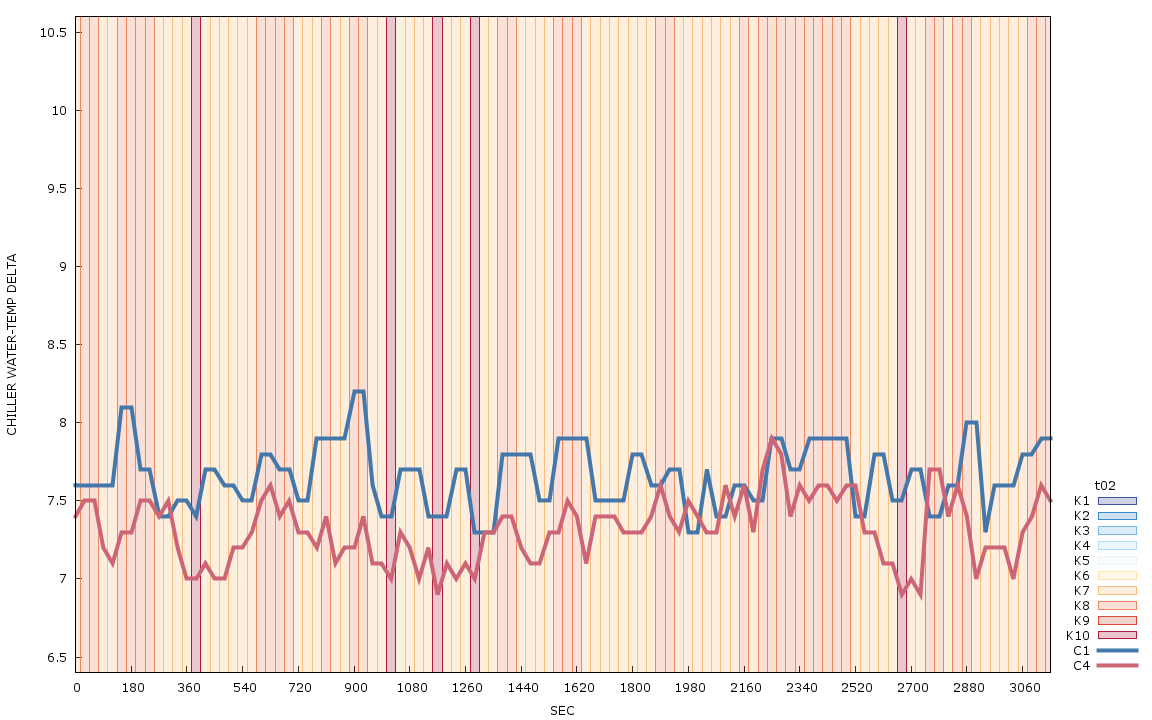
\includegraphics[bb=0 0 1152 720, width=15in]{cluster10/hd/CH_WTD/CH_WTD_t02.png}}
\fbox{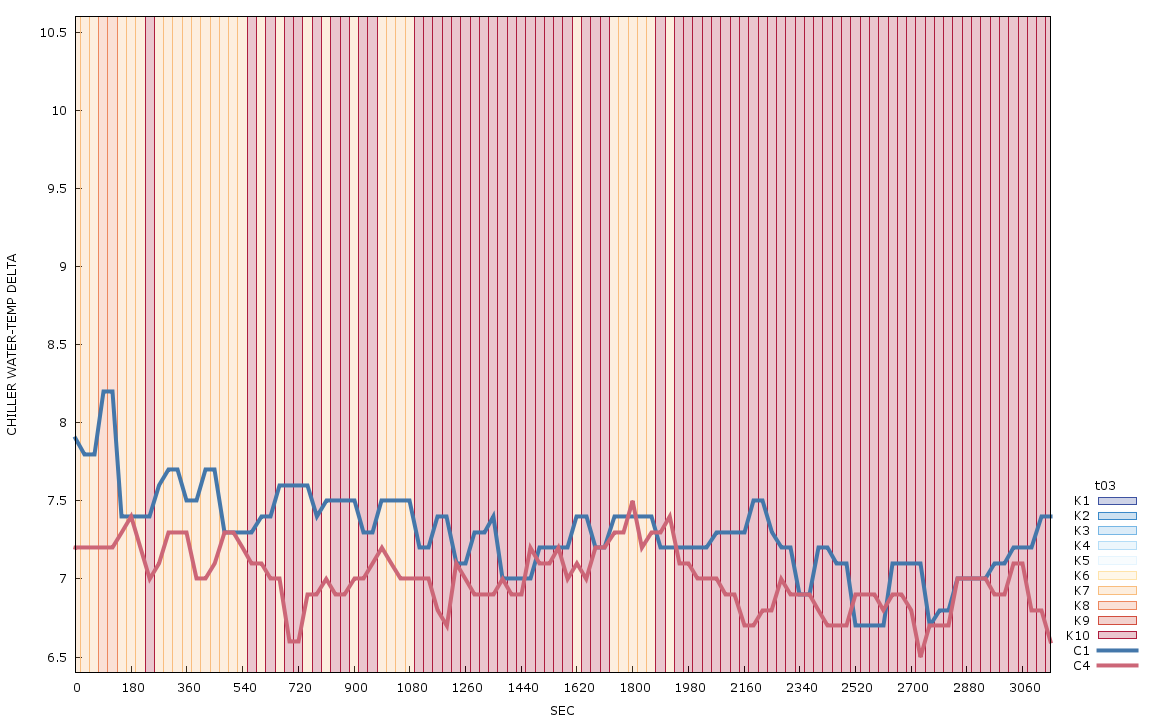
\includegraphics[bb=0 0 1152 720, width=15in]{cluster10/hd/CH_WTD/CH_WTD_t03.png}}
\caption{Chiller units C1 and C4; K-Means clustering across all three trials with $k=10$.}
\end{figure}
\begin{figure}[!h]
\centerline{\bfseries\large High-Density Workload : Trials 1--3}\\
\fbox{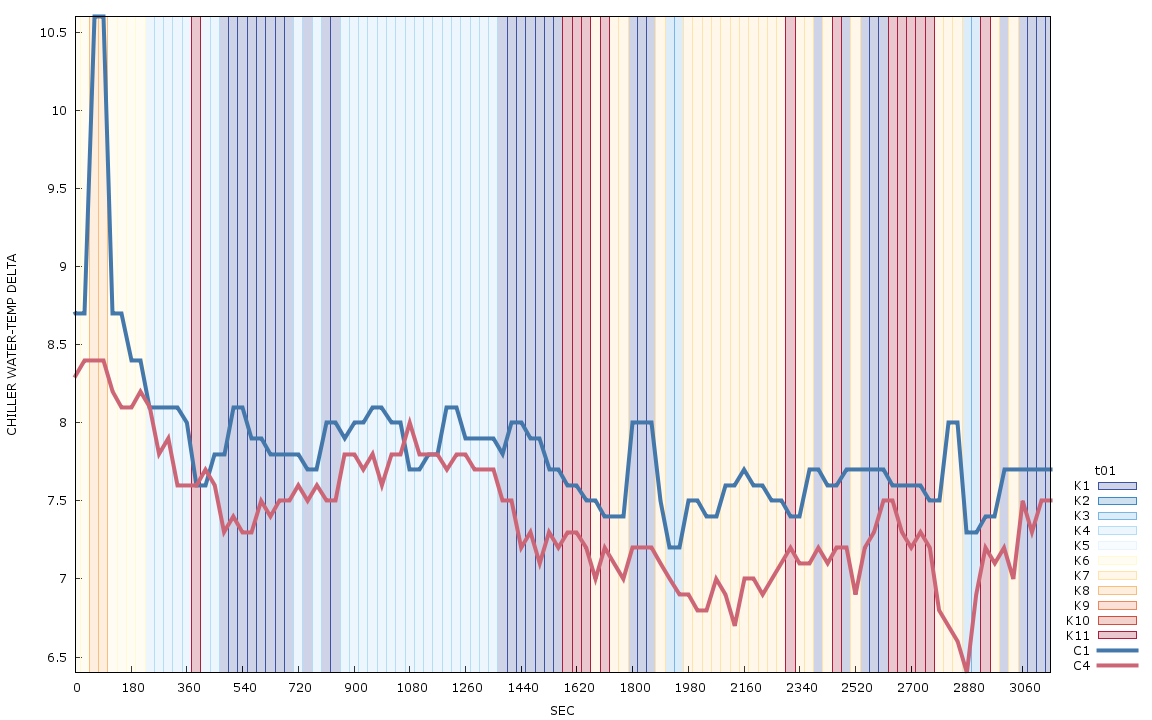
\includegraphics[bb=0 0 1152 720, width=15in]{cluster11/hd/CH_WTD/CH_WTD_t01.png}}
\fbox{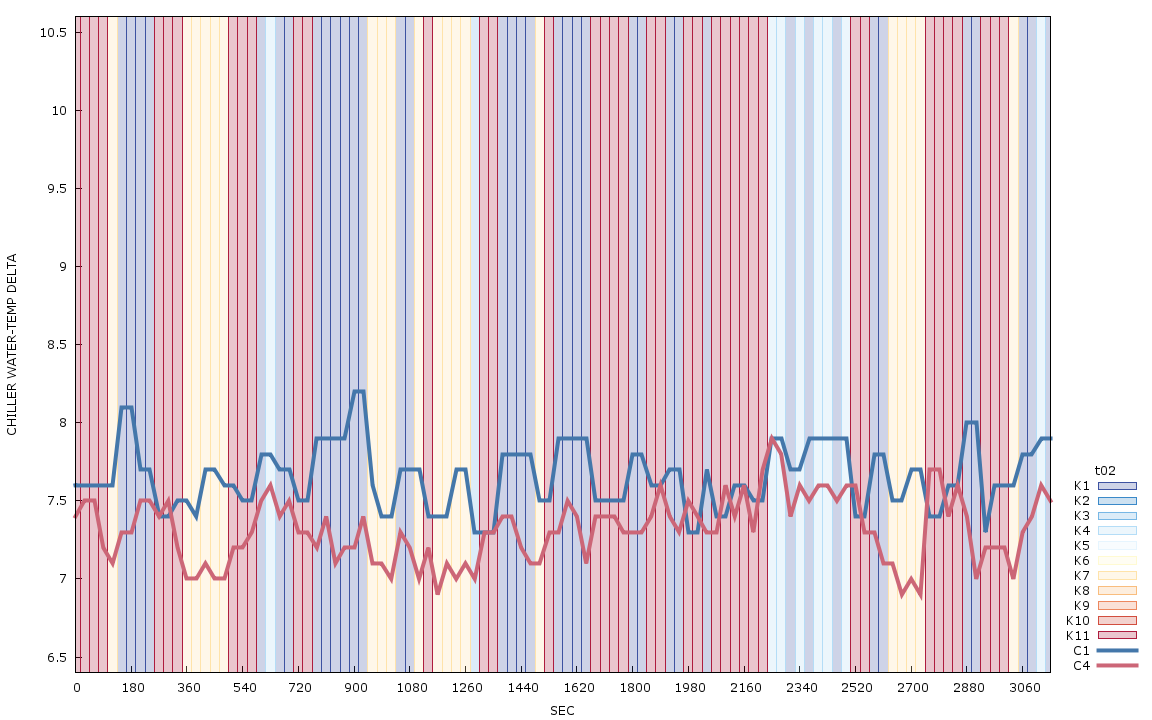
\includegraphics[bb=0 0 1152 720, width=15in]{cluster11/hd/CH_WTD/CH_WTD_t02.png}}
\fbox{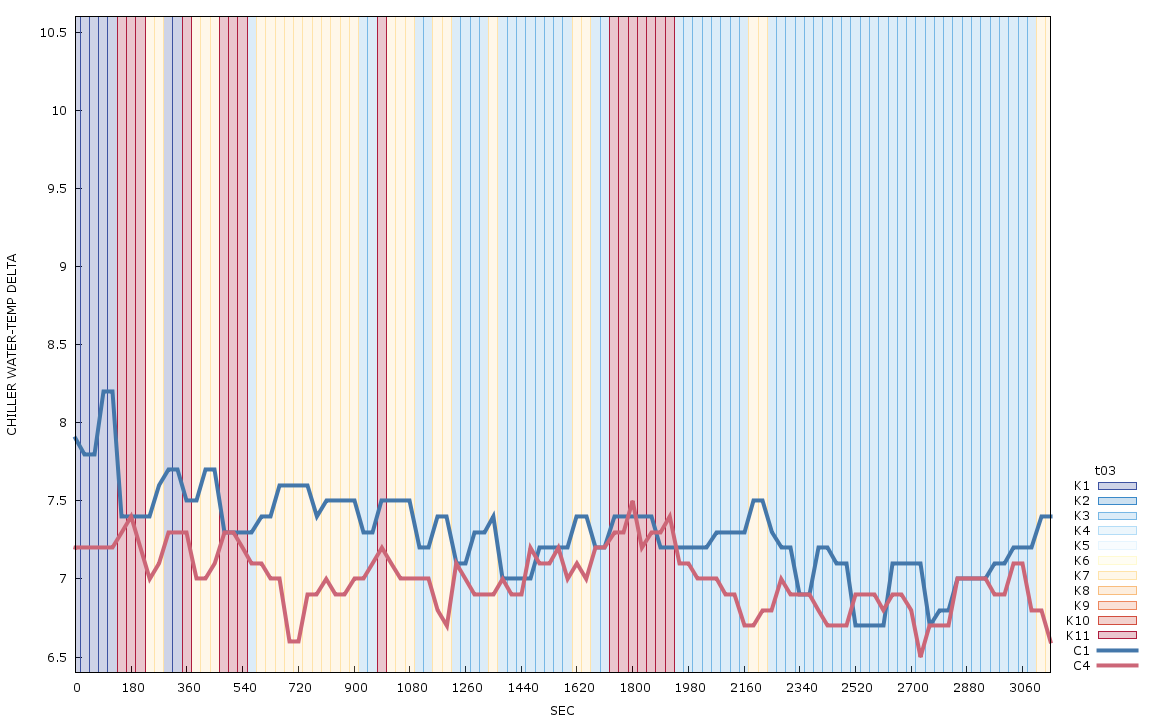
\includegraphics[bb=0 0 1152 720, width=15in]{cluster11/hd/CH_WTD/CH_WTD_t03.png}}
\caption{Chiller units C1 and C4; K-Means clustering across all three trials with $k=11$.}
\end{figure}
